\documentclass[unicode,12pt,a4paper,oneside,fleqn]{article}
\usepackage{styles/main} 
\ifpdf
    \hypersetup{
        pdffitwindow=false,
        pdfstartview={FitH},
        pdftitle={Курсовая работа за 5 курс},
        pdfauthor={Бедняков А.И.}
        pdfproducer={Бедняков А.И.},
        pdfsubject={Методы криптоанализа},
    }
\fi

\begin{document}
    \begin{titlepage}
    \begin{center}
        МИНОБРНАУКИ РОССИИ
        \linebreak

        \vspace{48pt}{
        Федеральное государственное бюджетное образовательное 
        учреждение высшего профессионального образования
        \linebreak
        «Ярославский государственный университет им. П.Г. Демидова»
        }
        \linebreak

        \vspace{1em}{
        Кафедра компьютерной безопасности и
        математических методов обработки информации
        }
    \end{center}

    \vspace{1em}

    \begin{center}
        \textsc{\textbf{Курсовая работа}}
        \linebreak
        \textsc{\textbf{«Реализация фреймворка для анализа криптограмм»}}
    \end{center}

    \vspace{6em}

	\begin{flushright}
        Научный руководитель \\
        \rule{2,2cm}{1pt} Белова Л.Ю. \\
        «\rule{0,5cm}{1pt}» \rule{2,5cm}{1pt} 2013 г.

        \vspace{1.5em}

        Студент группы КБ-51 \\
        \rule{2cm}{1pt} Бедняков А.И. \\
        «\rule{0,5cm}{1pt}» \rule{2,5cm}{1pt} 2013 г.
	\end{flushright}

    \vspace{\fill}

    \begin{center}
        Ярославль 2013
    \end{center}
\end{titlepage}

    \tableofcontents
    \pagebreak

    \begin{abstract}
Изучение методов защиты неразрывно связано с изучением 
возможных атак на алгоритмы и на их реализации. 
Работы по анализу таких шифров, как DES, ГОСТ 28147-89, Blowfish требуют 
большого ресурса и являются чрезвычайно сложными. 
В то же время на примерах классических шифров можно 
проиллюстрировать некоторые важные приемы и методы криптоанализа. 
После анализа классических шифров возможно изучение современных 
блочных алгоритмов шифрования, становятся доступными идеи 
линейного и дифференциального криптоанализа.

В этой работе предпринята попытка написания фреймворка 
для криптоанализа классических шифров и оценки стойкости 
современных шифров.
\end{abstract}

    \section{Введение}
    \DEF\textit{Лингвистика} (от лат. lingua — язык) — наука, это наука о 
всех языках мира как индивидуальных его представителях. В широком смысле 
слова, лингвистика подразделяется на научную и практическую.

\DEF\textit{Компьютерная лингвистика} — научное направление в области математического 
и компьютерного моделирования интеллектуальных процессов у человека и животных 
при создании систем искусственного интеллекта, которое ставит своей целью 
использование математических моделей для описания естественных языков.

\DEF\textit{Анализ текста} — процесс получения высококачественной информации из текста 
на естественном языке. Как правило, для этого применяется статистическое 
обучение на основе шаблонов: входной текст разделяется с помощью шаблонов,
затем производится обработка полученных данных.

Первоначально методы криптоанализа основывались на лингвистических закономерностях 
естественного текста и реализовывались с использованием только карандаша 
и бумаги. Со временем в криптоанализе нарастает роль чисто математических 
методов, для реализации которых используются специализированные криптоаналитические 
компьютеры.


    \pagebreak
    
    \section{Лингвистический и статистический анализ}
    \DEF\textit{Лингвистика} (от лат. lingua — язык) — наука, это наука о 
всех языках мира как индивидуальных его представителях. В широком смысле 
слова, лингвистика подразделяется на научную и практическую.

\DEF\textit{Компьютерная лингвистика} — научное направление в области математического 
и компьютерного моделирования интеллектуальных процессов у человека и животных 
при создании систем искусственного интеллекта, которое ставит своей целью 
использование математических моделей для описания естественных языков.

\DEF\textit{Анализ текста} — процесс получения высококачественной информации из текста 
на естественном языке. Как правило, для этого применяется статистическое 
обучение на основе шаблонов: входной текст разделяется с помощью шаблонов,
затем производится обработка полученных данных.

Первоначально методы криптоанализа основывались на лингвистических закономерностях 
естественного текста и реализовывались с использованием только карандаша 
и бумаги. Со временем в криптоанализе нарастает роль чисто математических 
методов, для реализации которых используются специализированные криптоаналитические 
компьютеры.


    \subsection{Словарный перебор}

Наиболее простой метод --- сравнение всех слов текста со словарем 
корректных слов нужного языка. Полученное количество совпавших слов
делится на количество слов исследуемого текста. Результирующая 
величина может рассматриваться как вероятность того, что данный 
текст принадлежит рассматриваемому языку.

Подобная оценка подходит целям данной работы --- критерий по 
этой 'вероятности' позволит отделить зерна от плевел и выделить 
наиболее пригодный вариант --- ложное срабатывание в общем случае 
маловероятно из-за специфики процесса. При негативном результате мы видим 
несвязный набор символов.

\begin{listing}[1]{1}
In [1]: import linguistics
In [2]: a = open('../sample/warandpeace', 'r').readlines()
In [3]: linguistics.istext_dict(a)
('ru', 0,864536523576)
\end{listing}

Здесь в первой строке подключается лингвистический модуль, 
во второй строке тестируемый текст записывается в переменную
$a$, и наконец в третьей вызывается метод определения языка 
по словарю. Метод возвращает предполагаемый язык и 
величину соответствия $V = \frac{n}{N}$, где $n$ --- количество
совпавших слов, а $N$ --- количество слов в тексте.

Практика демонстрирует жизнеспособность такого метода. Во-первых, 
составление 
словаря для известного языка в необходимой стилистике не представляет 
трудности при условии доступности интернета. Во-вторых, современные 
компьютерные мощности позволяют сравнительно быстрое выполнение 
подобного анализа:

\begin{listing}[1]{1}
# /usr/bin/time python ./cipher/linguistics.py -d ./sample/warandpeace 
python  710.10s user 780.55s system 0% cpu 20.002 total
\end{listing}

Здесь мы вызываем метод $istext\_dict$ через внешний 
интерфейс и отслеживаем время выполнения команды с помощью 
стандартной утилиты UNIX time.

Возможно совершествование данного метода путем написания более 
эффективных структур для хранения словаря, грамотной сериализации и 
использования оптимизированных алгоримов поиска по сортированному 
массиву. Но, как будет показано, в этом нет необходимости.
Во-первых мы не перешагнем известное ограничение сложности в 
$O(log(n))$ для алгоритмов поиска. Во-вторых, отсустствует необходимость 
в строгом соответствии текста языку определенному в словаре.
В-третьих, текст шифрограммы сравнительно редко содержит
пробелы, либо им нельзя доверять.

Но, эти пробелы возможно восстановить зная статистическое распределение
слов языка.
То есть необходимо на огромном объеме текста расчитать встречаемость
каждого слова и каждого словосочетания.
Такие данные сложно расчитать, но они уже были получены
в исследовании \cite{google-ngrams}.

Для примера, мы получили фразу \texttt{HELLOHOWAREYOUTODAY} и пытаемся 
определить наиболее вероятное разделение. Возможные разделения 
включают в себя:

\begin{verbatim}
HELLOHOWA REYOUTODAY
HELLO HOW ARE YOU TODAY
HE LL OH OW AR EY OU TO DA Y
H ELLOH OW AREYOU TOD AY
HELL OHO WARE YOU TODAY
\end{verbatim}

и многие другие.

\begin{listing}[1]{1}
In [1]: import cipher.linguistics as linguistics
In [2]: linguistics.restore_words('HELLOHOWAREYOUTODAY')
Out[2]: ['HELLO', 'HOW', 'ARE', 'YOU', 'TODAY']
\end{listing}

    \subsection{N-граммы}
N-грамма — последовательность из n элементов. С семантической точки зрения
, это может быть последовательность звуков, слогов, слов или букв. На практике 
чаще встречается N-грамма как ряд слов. Последовательность из двух последовательных 
элементов часто называют биграммы, последовательность из трех элементов 
называется триграмма. Не менее четырех и выше элементов обозначаются как 
N-грамма, N заменяется на количество последовательных элементов.


    \pagebreak

    \section{Криптоанализ классических шифров}
    \DEF\textit{Лингвистика} (от лат. lingua — язык) — наука, это наука о 
всех языках мира как индивидуальных его представителях. В широком смысле 
слова, лингвистика подразделяется на научную и практическую.

\DEF\textit{Компьютерная лингвистика} — научное направление в области математического 
и компьютерного моделирования интеллектуальных процессов у человека и животных 
при создании систем искусственного интеллекта, которое ставит своей целью 
использование математических моделей для описания естественных языков.

\DEF\textit{Анализ текста} — процесс получения высококачественной информации из текста 
на естественном языке. Как правило, для этого применяется статистическое 
обучение на основе шаблонов: входной текст разделяется с помощью шаблонов,
затем производится обработка полученных данных.

Первоначально методы криптоанализа основывались на лингвистических закономерностях 
естественного текста и реализовывались с использованием только карандаша 
и бумаги. Со временем в криптоанализе нарастает роль чисто математических 
методов, для реализации которых используются специализированные криптоаналитические 
компьютеры.


    \subsection{Шифр Цезаря}

Шифр Цезаря — это вид шифра подстановки, в котором каждый символ в открытом тексте заменяется буквой находящейся на некоторое постоянное число позиций левее или правее него в алфавите. Например, в шифре со сдвигом 3 А была бы заменена на Г, Б станет Д, и так далее.

Шифр назван в честь римского императора Гая Юлия Цезаря, использовавшего его для секретной переписки со своими генералами.

\subsubsection{Описание}

Если сопоставить каждому символу алфавита его порядковый номер (нумеруя с 0), то шифрование и дешифрование можно выразить формулами модульной арифметики:

    $$y=(x+k)\ \mod\ n$$
    $$x=(y-k+n)\ \mod\ n,$$

где $x$ — символ открытого текста, $y$ — символ шифрованного текста, $n$ — мощность алфавита, а $k$ — ключ.

\subsubsection{Криптоанализ}

Шифр Цезаря может быть легко взломан даже в случае, когда взломщик знает только зашифрованный текст. Можно рассмотреть две ситуации:

1. взломщик знает (или предполагает), что использовался простой шифр подстановки, но не знает, что это — схема Цезаря;

2. взломщик знает, что использовался шифр Цезаря, но не знает значение сдвига.

В первом случае шифр может быть взломан, используя те же самые методы что и для простого шифра подстановки, такие как частотный анализ и т. д., Используя эти методы, взломщик, вероятно, быстро заметит регулярность в решении и поймёт, что используемый шифр — это шифр Цезаря.

Во втором случае, взлом шифра является даже более простым. Существует не так много вариантов значений сдвига (26 для английского языка), все они могут быть проверены методом грубой силы. Один из способов сделать это — выписать отрывок зашифрованного текста в столбец всех возможных сдвигов — техника, иногда называемая как «завершение простого компонента». Рассмотрим пример для зашифрованного текста «EXXEGOEXSRGI»; открытый текст немедленно опознается глазом в четвертой строке.

Другой способ применения этого метода — это написать алфавит под каждой буквой зашифрованного текста, начиная с этой буквы. Метод может быть ускорен, если использовать заранее подготовленные полоски с алфавитом. Для этого нужно сложить полоски так, чтобы в одной строке образовался зашифрованый текст, тогда в некоторой другой строке мы увидим открытый текст.

Для обычного текста на естественном языке, скорее всего, будет только один вариант декодирования. Но, если использовать очень короткие сообщения, то возможны случаи, когда возможны несколько вариантов расшифровки с различными сдвигами. Например зашифрованный текст MPQY может быть расшифрован как «aden» так и как «know» (предполагая, что открытый текст написан на английском языке). Точно также «ALIIP» можно расшифровать как «dolls» или как «wheel»; «AFCCP» как «jolly» или как «cheer».

Многократное шифрование никак не улучшает стойкость, так как применение шифров со сдвигом a и b эквивалентно применению шифра со сдвигом a+b. В математических терминах шифрование с различными ключами образует группу.

    \subsection{Аффинный шифр}

Аффинный шифр — это частный случай более общего моноалфавитного шифра 
подстановки. К шифрам подстановки относятся также шифр Цезаря, 
ROT13 и Атбаш. Поскольку аффинный шифр легко дешифровать, 
он обладает слабыми криптографическими свойствами.

\subsubsection{Описание}

В аффинном шифре каждой букве алфавита размера m ставится в 
соответствие число из диапазона $[0, ..., m - 1]$. 
Затем при помощи модульной арифметики для каждого числа, соответствующего 
букве исходного алфавита, вычисляется новое число, которое заменит 
старое в шифротексте. Функция шифрования для каждой буквы

    $$\mbox{E}(x) = (ax + b) \mod{m},$$

где модуль $m$ — размер алфавита, а пара $a$ и $b$ — ключ шифра. Значение 
$a$ должно быть выбрано таким, что $a$ и $m$ — взаимно простые числа. Функция 
расшифрования

    $$\mbox{D}(x) = a^{-1} \times (x - b) \mod{m},$$

где $a^{-1}$ — обратное к $a$ число по модулю $m$. То есть оно удовлетворяет 
уравнению

    $$1 \equiv a \times a^{-1} \mod{m}.$$

Обратное к $a$ число существует только в том случае, когда $a$ и $m$ — взаимно 
простые. Значит, при отсутствии ограничений на выбор числа $a$ расшифрование 
может оказаться невозможным. Покажем, что функция расшифрования является 
обратной к функции шифрования:

\begin{equation}
    \begin{matrix}
        \mbox{D}(\mbox{E}(x)) 
          &= &a^{-1} \times (\mbox{E}(x) - b) \mod{m} \\ 
          &= &a^{-1} \times ((ax + b) - b) \mod{m} \\ 
          &= &a^{-1} \times (ax + b - b) \mod{m} \\ 
          &= &a^{-1} \times ax \mod{m}\\ 
          &= &x \mod{m}. 
    \end{matrix}
\end{equation}

Количество возможных ключей для аффинного шифра можно записать 
с помощью функции Эйлера как $\varphi(m) \times m$.

\subsubsection{Криптоанализ, минимизация вариантов перебора}

Так как аффинный шифр является по сути моноалфавитным шифром замены
, то он обладает всеми уязвимостями этого класса шифров. Шифр Цезаря —
это аффинный шифр с $a = 1$, что сводит функцию шифрования к простому 
линейному сдвигу.

В случае шифрования сообщений на русском языке (т. е. с помощью $m = 33$) 
существует 627 нетривиальных аффинных шифров, не учитывая 33 тривиальных шифра 
Цезаря. Это число легко посчитать, зная, что существует всего 20 чисел 
взаимно простых с 33 и меньших 33 (а это и есть возможные значения 
$a$). Каждому значению a могут соответствовать 33 разных дополнительных 
сдвига (значение $b$); то есть всего существует 2033 или 660 возможных 
ключей. Аналогично, для сообщений на английском языке (т.е. $m = 26$) 
всего существует 1226 или 312 возможных ключей. Такое ограниченное 
количество ключей приводит к тому, что система крайне не криптостойка 
с точки зрения принципа Керкгоффса.

Основная уязвимость шифра заключается в том, что криптоаналитик может 
выяснить (путем частотного анализа, полного перебора, угадывания или 
каким-либо другим способом) соответствие между двумя любыми буквами 
исходного текста и шифротекста. Тогда ключ может быть найдет путем 
решения системы уравнений. Кроме того, так мы знаем, что $a$ и $m$ — взаимно 
простые, это позволяет уменьшить количество проверяемых ключей для 
полного перебора.

\begin{listing}[1]{1}
def decipher(self, iteration = 0, shift = 0):
    base = range(1, len(self.alphabet) + 1)
    for a in base:
        coprimes = [b for b in base if cipher.routine.gcd(a, b) == 1]
        for b in coprimes:
            ot = self.decrypt(a, b)
            if self.istext(ot) > 0.7:
                return (ot, a, b)
\end{listing}

Преобразование, подобное аффинному шифру, используется в линейном 
конгруэнтном методе (разновидности генератора псевдослучайных чисел).
Этот метод не является криптостойким по той же причине, что и аффинный 
шифр.

\begin{figure}[bh]
\noindent\centering{
    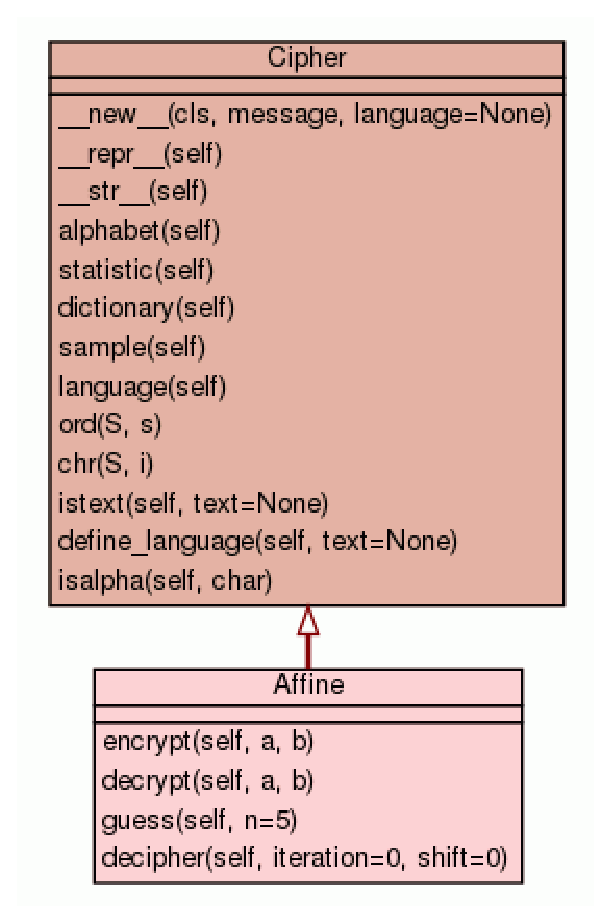
\includegraphics[width=65mm]{\globalImages/uml_affine.eps}
}
\caption{UML диаграмма класса анализа афинного шифра}
\label{figCurves}
\end{figure}

Диаграмма показывает, что афинный шифр успено вписывается 
в разработанную архитектуру.

    \subsection{Шифр Виженера}

Шифр Виженера --- метод полиалфавитного 
шифрования буквенного текста с использованием ключевого слова.

Этот метод является простой формой многоалфавитной замены. Шифр 
Виженера изобретался многократно. Впервые этот метод описал
Giovan Battista Bellaso) в 1553 году, однако в XIX веке 
получил имя Блеза Виженера, французского дипломата. Метод прост 
для понимания и реализации, он является недоступным для простых 
методов криптоанализа.

Первое точное документированное описание многоалфавитного шифра 
было сформулированно Леоном Баттиста Альберти в 1467 году, для 
переключения между алфавитами использовался металлический шифровальный 
диск. Система Альберти переключает алфавиты после нескольких 
зашифрованных слов. Позднее, в 1518 году, Иоганн Трисемус в своей 
работе «Полиграфия» изобрел tabula recta — центральный компонент 
шифра Виженера.

Блез Виженер представил свое описание простого, но стойкого шифра 
перед комиссией Генриха III во Франции в 1586 году, и позднее 
изобретение шифра было присвоено именно ему. Давид Кан в своей 
книге «Взломщики кодов» отозвался об этом осуждающе, написав, 
что история «проигнорировала важный факт и назвала шифр именем 
Виженера, несмотря на то, что он ничего не сделал для его создания».

Шифр Виженера имел репутацию исключительно стойкого к «ручному»
взлому. Известный писатель и математик Чарльз Лютвидж Доджсон 
(Льюис Кэрролл) назвал шифр Виженера невзламываемым в своей статье 
«Алфавитный шифр», опубликованной в 
детском журнале в 1868 году. В 1917 году Scientific American 
также отозвался о шифре Виженера, как о неподдающемся взлому. 
Это представление было опровергнуто после того, как Касиски полностью 
взломал шифр в XIX веке, хотя известны случаи взлома этого шифра 
некоторыми опытными криптоаналитиками еще в XVI веке.

\subsubsection{Описание шифра Виженера}

В шифре Цезаря каждая буква алфавита сдвигается на несколько 
строк; например в шифре Цезаря при сдвиге +3, A стало бы D, B 
стало бы E и так далее. Шифр Виженера состоит из последовательности 
нескольких шифров Цезаря с различными значениями сдвига. Для 
зашифровывания может использоваться таблица алфавитов, называемая 
tabula recta или квадрат (таблица) Виженера. Применительно к 
латинскому алфавиту таблица Виженера составляется из строк по 
26 символов, причём каждая следующая строка сдвигается на несколько 
позиций. Таким образом, в таблице получается 26 различных шифров 
Цезаря. На разных этапах кодировки шифр Виженера использует различные 
алфавиты из этой таблицы. На каждом этапе шифрования используются 
различные алфавиты, выбираемые в зависимости от символа ключевого 
слова. Например, предположим, что исходный текст имеет вид:

\begin{verbatim}
                               ATTACKATDAWN
\end{verbatim}

Человек, посылающий сообщение, записывает ключевое слово («LEMON») 
циклически до тех пор, пока его длина не будет соответствовать 
длине исходного текста:

\begin{verbatim}
                               LEMONLEMONLE
\end{verbatim}

Первый символ исходного текста A зашифрован последовательностью 
L, которая является первым символом ключа. Первый символ L шифрованного 
текста находится на пересечении строки L и столбца A в таблице 
Виженера. Точно так же для второго символа исходного текста используется 
второй символ ключа; то есть второй символ шифрованного текста 
X получается на пересечении строки E и столбца T. Остальная часть 
исходного текста шифруется подобным способом.

\begin{verbatim}
                               ATTACKATDAWN
                               LEMONLEMONLE
                               LXFOPVEFRNHR
\end{verbatim}

Расшифровывание производится следующим образом: находим в таблице 
Виженера строку, соответствующую первому символу ключевого слова;
в данной строке находим первый символ зашифрованного текста.
Столбец, в котором находится данный символ, соответствует первому 
символу исходного текста. Следующие символы зашифрованного текста 
расшифровываются подобным образом.

Если буквы A-Z соответствуют числам 0-25, то шифрование и 
расшифрование Виженера 
можно записать в виде формул:

    $$C_i \equiv (P_i + K_i) \mod\ 26$$
    $$P_i \equiv (C_i - K_i + 26) \mod\ 26$$

\subsubsection{Криптоанализ, работа с полиалфавитными шифрами}

Шифр Виженера «размывает» характеристики частот появления символов 
в тексте, но некоторые особенности появления символов в тексте 
остаются. Главный недостаток шифра Виженера состоит в том, что 
его ключ повторяется. Поэтому простой криптоанализ шифра может 
быть построен в два этапа:

Поиск длины ключа. Можно анализировать распределение частот в 
зашифрованном тексте с различным прореживанием. То есть брать 
текст, включающий каждую 2-ю букву зашифрованного текста, потом 
каждую 3-ю и т. д. Как только распределение частот букв будет 
сильно отличаться от равномерного (например, по энтропии), то 
можно говорить о найденной длине ключа.

\paragraph{Метод Касиски}

В 1863 году Фридрих Касиски был первым, кто опубликовал успешный 
алгоритм атаки на шифр Виженера, хотя Чарльз Беббидж разработал 
этот алгоритм уже в 1854 году. В то время когда Беббидж занимался 
взломом шифра Виженера, John Hall Brock Thwaites представил новый 
шифр в «Journal of the Society of the Arts»; когда Беббидж показал,
что шифр Thwaites’а является лишь частным случаем шифра Виженера,
Thwaites предложил ему его взломать. Беббидж расшифровал текст,
который оказался поэмой «The Vision of Sin» Альфреда Теннисона,
зашифрованной ключевым словом Emily — именем жены поэта.

Тест Касиски опирается на то, что некоторые слова, такие как 
«the» могут быть зашифрованы одинаковыми символами, что приводит 
к повторению групп символов в зашифрованном тексте. Например: 
сообщение, зашифрованное ключом ABCDEF , не всегда одинаково 
зашифрует слово «crypto».

Зашифрованный текст в данном случае не будет повторять последовательности 
символов, которые соответствуют повторным последовательностям 
исходного текста. В данном шифрованном тексте есть несколько 
повторяющихся сегментов, которые позволяют криптоаналитику найти 
длину ключа.

Более длинные сообщения делают тест более точным, так как они 
включают в себя больше повторяющихся сегментов зашифрованного 
текста. В данном шифрованном тексте есть несколько повторяющихся 
сегментов, которые позволяют криптоаналитику найти длину ключа.

Расстояние между повторяющимися DYDUXRMH равно 18, это позволяет 
сделать вывод, что длина ключа равна одному из значений: 
18, 9, 6, 3 или 2. Расстояние между повторяющимися NQD равно 20. Из 
этого следует, что длина ключа равна 20, 10, 5, 4 
или 2. Сравнивая возможные длины ключей, можно сделать вывод, 
что длина ключа (почти наверняка) равна 2.

\paragraph{Тест Фридмана}

(иногда называемый каппа-тест) был изобретен Вильямом 
Фридманом в 1920 году. Фридман использовал индекс совпадения, 
который измеряет частоты повторения символов, чтобы взломать 
шифр. Зная вероятность $\kappa_p$ того, что два случайно выбранных 
символа текста совпадают (примерно 0,067 для англ. языка) и вероятность 
совпадения двух случайно выбранных символов алфавита $\kappa_r$ 
(примерно 1 / 26 = 0,0385 для англ. языка), можно оценить длину 
ключа как:

    $${\kappa_p-\kappa_r}\over{\kappa_o-\kappa_r}$$

Из наблюдения за частотой совпадения следует:

    $$\kappa_o=\frac{\sum_{i=1}^{c}n_i(n_i -1)}{N(N-1)}$$

Где $С$ — размер алфавита (26 символов для англ. языка), $N$ — длина 
текста, и $n_1$ до $n_c$ — наблюдаемые частоты повторения символов 
зашифрованного текста. Однако, это только приблизительное значение,
точность которого увеличивается при большем размере текста. 
На практике это было бы необходимо для перебора различных ключей 
приближаясь к исходному.

\paragraph{Частотный анализ}

Как только длина ключа становится известной, зашифрованный текст 
можно записать во множество столбцов, каждый из которых соответствует 
одному символу ключа. Каждый столбец состоит из исходного текста
, который зашифрован шифром Цезаря; ключ к шифру Цезаря является 
всего-навсего одним символом ключа для шифра Виженера, который 
используется в этом столбце. Используя методы, подобные методам 
взлома шифра Цезаря, можно расшифровать зашифрованный текст. 
Усовершенствование теста Касиски, известное как метод Кирхгофа
, заключается в сравнении частоты появления символов в столбцах 
с частотой появления символов в исходном тексте для нахождения 
ключевого символа для этого столбца. Когда все символы ключа 
известны, криптоаналитик может легко расшифровать шифрованный 
текст, получив исходный текст. Метод Кирхгофа не применим, когда 
таблица Виженера скремблирована, вместо использования обычной 
алфавитной последовательности, хотя тест Касиски и тесты совпадения 
всё ещё могут использоваться для определения длины ключа для 
этого случая.

    \subsection{Энигма}

\paragraph{Описание}

\paragraph{Криптоанализ}

    \pagebreak

    \section{Криптоанализ бинарных шифров}
    \DEF\textit{Лингвистика} (от лат. lingua — язык) — наука, это наука о 
всех языках мира как индивидуальных его представителях. В широком смысле 
слова, лингвистика подразделяется на научную и практическую.

\DEF\textit{Компьютерная лингвистика} — научное направление в области математического 
и компьютерного моделирования интеллектуальных процессов у человека и животных 
при создании систем искусственного интеллекта, которое ставит своей целью 
использование математических моделей для описания естественных языков.

\DEF\textit{Анализ текста} — процесс получения высококачественной информации из текста 
на естественном языке. Как правило, для этого применяется статистическое 
обучение на основе шаблонов: входной текст разделяется с помощью шаблонов,
затем производится обработка полученных данных.

Первоначально методы криптоанализа основывались на лингвистических закономерностях 
естественного текста и реализовывались с использованием только карандаша 
и бумаги. Со временем в криптоанализе нарастает роль чисто математических 
методов, для реализации которых используются специализированные криптоаналитические 
компьютеры.


    \subsection{XOR}

XOR --- это побитовое сложение по модулю 
(с инвертированием при переполнении), 
например, $1+1=0$ т.к. $1$ - максимальное значение. Все варианты:

$$0 \oplus 0=0$$
$$0 \oplus 1=1$$
$$1 \oplus 1=0$$

\subsubsection{Описание шифра XOR}

То есть, операция $z = x \oplus y$ по сути поразрядная (побитовая — 
результат не зависит от соседних битов). Если только один из 
соответствующих битов равен 1, то результат 1. А если оба 0 или 
оба 1, то результат 0. Если внимательно посмотреть на результат 
применения XOR к двум двоичным числам, то можно заметить, что 
мы можем восстановить одно из слагаемых при помощи второго: $x 
= z \oplus y$ или $y = z \oplus x$. 

\subsubsection{Криптоанализ, интерпретация бинарных данных}

Отсюда можно сделать следующие выводы: зная число y и применяя 
XOR к $x$, мы получим $z$. Затем, мы, опять же используя $y$, получим 
из $z$ обратно число $x$. Таким образом мы можем преобразовать последовательность 
чисел $(x)_i$ в последовательность $(z)_i$. Теперь мы можем назвать 
число y кодирующим (или шифрующим) ключом. Если человек не знает 
ключа, то он не сможет восстановить исходную последовательность 
чисел $(x)_i$.

Поскольку каждая буква будет представлена в шифротексте 
одним и тем же кодом $z$, то пользуясь частотным словарем взломщик 
сможет вычислить шифрующий ключ $y$, если у него будет в распряжениии 
достаточно длинный шифротекст. 
\begin{figure}[H]
\noindent\centering{
    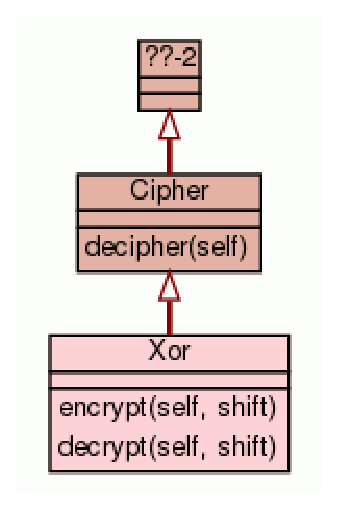
\includegraphics[width=35mm]{\globalImages/uml_xor.eps}
}
\caption{UML диаграмма класса анализа шифра XOR}
\label{uml_xor}
\end{figure}

В случае длинного ключа применяются уже разобранные методы 
анализа из шифра Виженера. 
Структура класса для анализа шифра Xor
представлена на диаграмме \ref{uml_xor}.

    \pagebreak

    \section{Приложения}
\begin{appendix}
    \subsection{Исходный код}
        %\begin{enumerate}
            %\item{Функция верификации пароля}
            %\lstinputlisting{./code/motc-checker}
            %\item{Функция идентификации пользователя}
            %\lstinputlisting{./code/motc-id}
        %\end{enumerate}

    %\subsection{Блок-схема}
        %\includegraphics[width=160mm]{./img/atmel.png}
\end{appendix}

\pagebreak

    \addcontentsline{toc}{section}{Список литературы}
\begin{thebibliography}{1}

\bibitem{andersonbondcryptoprocessors} Anderson R., Bond M., ``Cryptographic processors – a survey'' // Proceedings of the IEEE, с 357—369, 2006.
\bibitem{catheydowskinewparadigm} W.T. Cathey and E.R. Dowski, ``New paradigm for imaging systems'', Appl. Opt. 41, pp. 6080-6092, 2002.
\bibitem{skorobogatovsidechannelattacks} Skorobogatov S., ``Side-channel attacks: new directions and horizons'' // Design and Security of Cryptographic Algorithms and Devices (ECRYPT II), 2011
\bibitem{gandolfielectromagnectic} Gandolfi K. , Naccache D. ``Electromagnetic Analysis: Concrete Results'' // Proceedings of the Third International Workshop on Cryptographic Hardware and Embedded Systems, Springer-Verlag, с. 251—261, 2001.
\bibitem{shnayerprikladnayakripto} Шнайер Б., ``Прикладная криптография. Протоколы, алгоритмы, исходные тексты на языке Си'', М.: Триумф, 2002. — 816 с.
\end{thebibliography}

\end{document}

